\subsection{Feature extraction and selection}
The training set has been built starting from the preprocessed tweets, characterized by 788 tweets classified as 'body shaming' and 788 other tweets 'non-body shaming'.
Using the \emph{sklearn.feature\_extraction} library of Python every model has been integrated as the last step of pipeline composed by the following steps:

\begin{itemize}
\item \textbf{vectorization} using CountVectorizer() with ngram = 1 the collection of tweets is converted to a matrix of token counts;
\item  \textbf{Tf-Idf}: This weight is a statistical measure used to evaluate how important a word (stem) is to a document (tweet) in a collection or corpus. The importance increases proportionally to the number of times a word appears in the document but is offset by the frequency of the word in the corpus (data-set);
\item \textbf{feature selection} using SelectPercentile() with \emph{percentage} parameter equal to 75, a number of features equal to about 3500, with respect to the initial 4669, has been obtained. \end{itemize}

\noindent
For the feature selection phase, different values of percentage have been compared.


\begin{figure}[H]
\centering
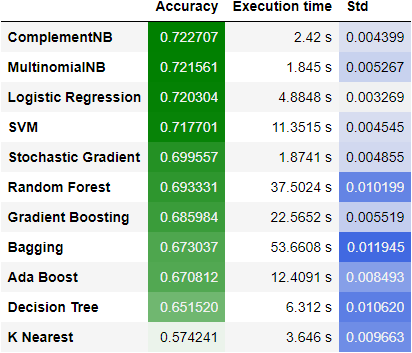
\includegraphics[width=.47\textwidth]{images/features/cross_val_result_75.png}\hfil
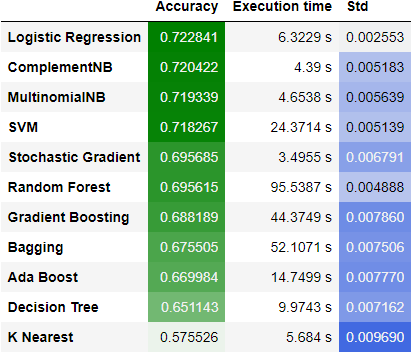
\includegraphics[width=.47\textwidth]{images/features/cross_val_result_85.png}

\caption{Percentage of feature selection compared: 75\%, 85\%}\label{fig:75-85}
\end{figure}

\noindent
As shown in the table \ref{fig:75-85}, regardless of the percentage of selected features, the 4 classifiers that perform best are: \emph{Logistic Regression}, \emph{SVM}, \emph{ComplementNB} and \emph{MultinomialNB}. These algorithms have the best accuracy and lowest standard deviation. Considering the execution times all perform well except for SVM that is the slowest.

Changing the feature percentage the accuracy does not change a lot therefore, focusing on \emph{Logistic Regression}, \emph{ComplementNB} and \emph{MultinomialNB}, the standard deviation and the execution times are lower with a value of 75\% that allows to lighten the computation.
Moreover, in this scenario the best 4 classifiers will be compared with some metrics.